% !TeX encoding = UTF-8
\section{Anhang}

\begin{figure}[h]
    \centering
    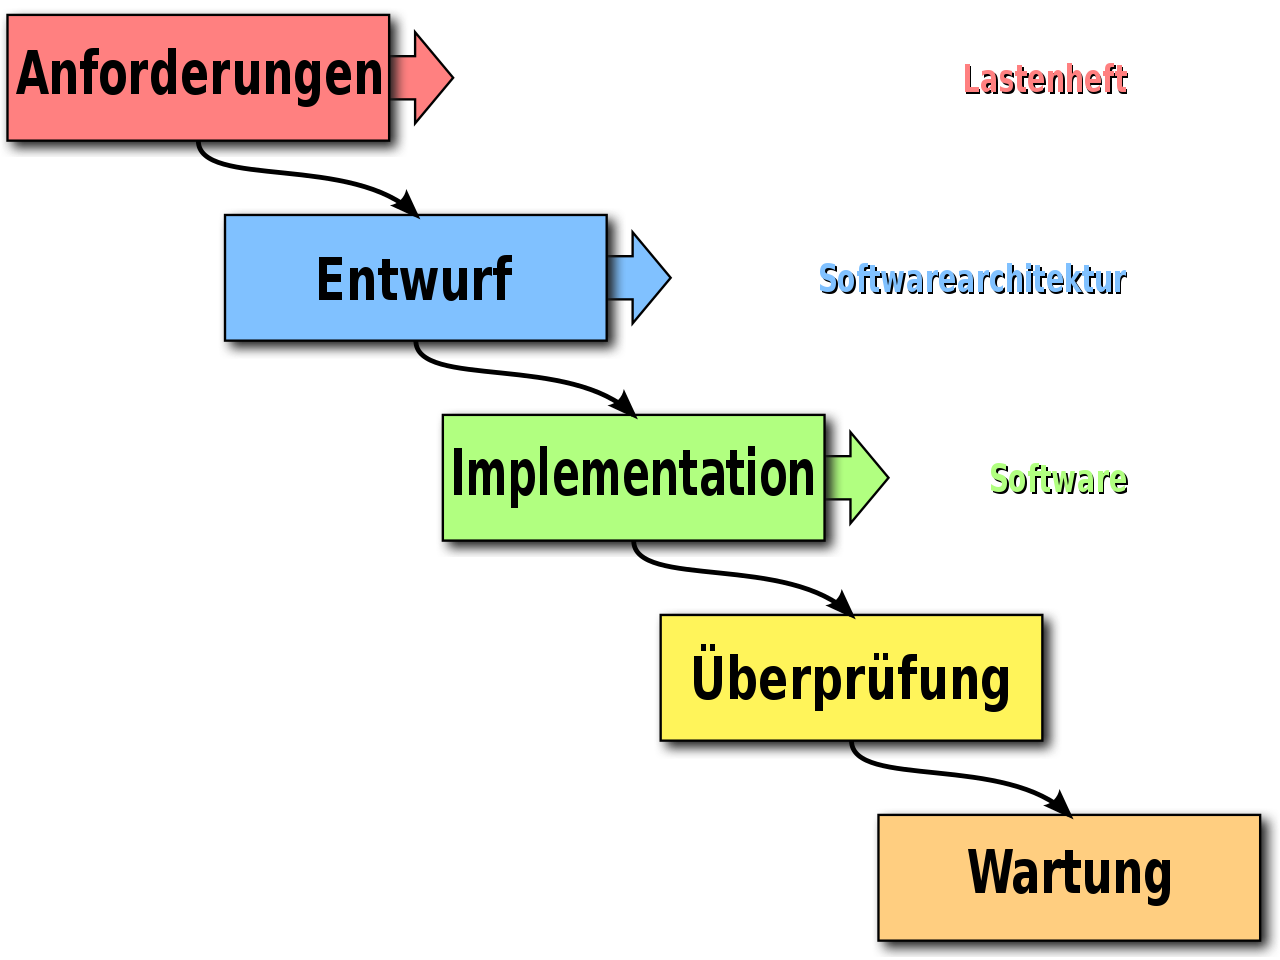
\includegraphics[width=0.7\textwidth]{res/Waterfall_model-de.svg.png} 
    \caption{Ablauf der Softwareentwicklung nach dem Wasserfallmodell} \cite{wasserfallmodellPic}
    \label{fig:wasserfallmodell}
\end{figure}

As you can see in the figure \ref{fig:wasserfallmodell}, the 
function grows near 0. Also, in the page \pageref{fig:wasserfallmodell} 
is the same example.

\myNewSection
\textbf{Stichpunkte:} 
Ermüdende Informationsberge sollten in einen Anhang verbannt werden. (Wichtige Begriffe definieren)

%Beispiel: passende Lösung für dieses Problem zu finden
\myNewSection \label{anhang:einleitung:passendeLösung}
Um diese Idee \dq Stärken des Pc's sowie des Handys zu nutzen\dq noch etwas verständlicher zu machen, folgt eine kurzes Beispiel, wie diese Idee zu einem erfolgreichen Produkt geführt hat.
Der erste Ipod\cite{einleitung_ipod} wurde 2001 vorgestellt und als \glqq tragbarer digitaler Medienabspielgeräte\grqq{} entworfen. Der Kleinheit und Portabilität zugunsten wurden nur die für das Gerät passenden und nötigen Funktionen implementiert. So zum Beispiel das Abspielen und Auswählen von Musik. Funktionen welche auf solch einem kleinen Gerät nicht gut funktionieren, wurden auf den Pc verlagert. So war der Pc für eine seiner Stärken zuständig, und zwar der Konfiguration, also dem Hinzufügen, Bearbeiten und Löschen von Musik. 